\section{Servicios de Persistencia}

Si bien para la persistencia de los datos creamos los manejadores de archivos, es necesario un objeto que se encargue de administrar el acceso y la recuperaci�n de los mismos a un nivel mayor de abstracci�n, es decir, a nivel de palabras y sonidos.
Es necesario, adem�s, de acuerdo a los requerimientos de entregas posteriores, que su interfaz sea independiente de la implementaci�n de los archivos.
  
\subsection{Requerimientos del servicio de persistencia}

El servicio de persistencia encapsula el manejo de los dos archivos: el de palabras y el del audio. Debe presentar una interfaz que permita agregar palabras con su respectivo audio, consultar si una palabra est� registrada y recuperar un audio a partir de su correspondiente palabra.
Decidimos que una vez que la palabra fue registrada, no s�lo no se pueda eliminar, sino que adem�s, no se puede modificar su registro de audio. En este caso, el servicio debe informar que no es una acci�n v�lida.

\subsection{Implementaci�n del servicio de persistencia}

De acuerdo a los requerimientos mencionados anteriormente, definimos que el servicio de persistencia debe implementar la interfaz \textbf{SoundPersistenceService}.
En particular, para esta entrega, la clase \textbf{SoundPersistenceServiceVariableLengthImpl} lo hace utilizando archivos con registros de longitud variable organizados en bloques.

En la siguiente im�gen podemos observar las caracter�sticas de esta interfaz y, posteriormente, analizaremos la implementaci�n:

\begin{figure}[!htp]
	\begin{center}
		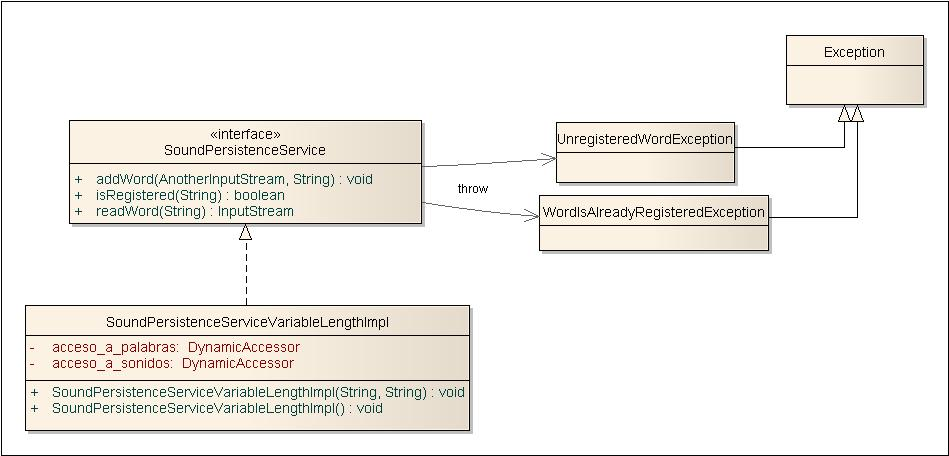
\includegraphics[scale=0.5]{img/ClassModelSoundService2.JPEG}
	\end{center}
	\caption{Diagrama de clases del SoundPersistenceService}} 
	\label{fig:classSPS1}
\end{figure}
 

\begin{figure}[!htp]
	\begin{center}
		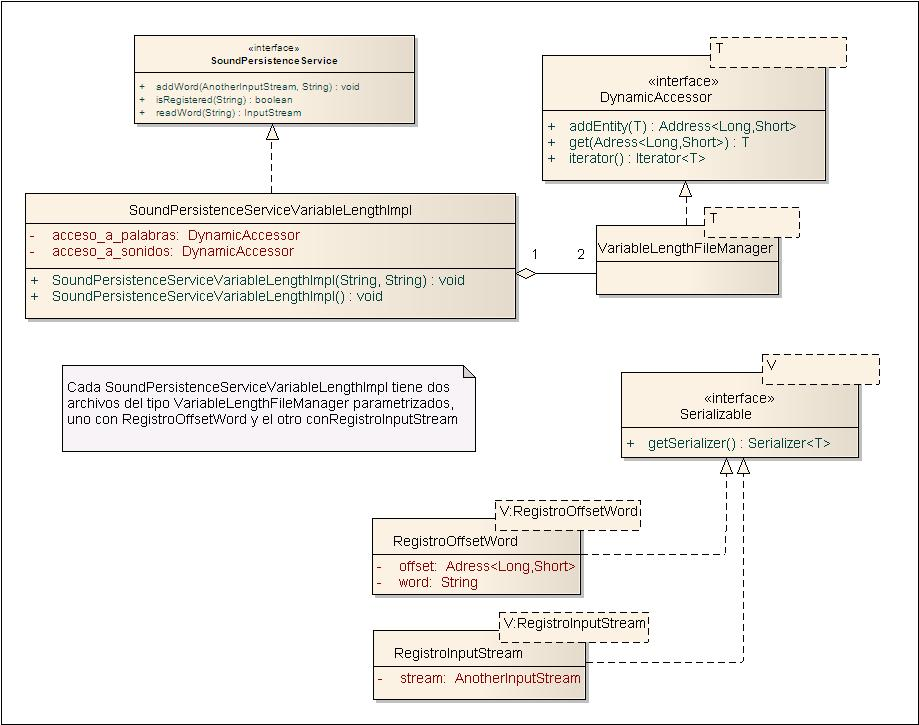
\includegraphics[scale=0.5]{img/ClassModelSoundService1.JPEG}
	\end{center}
	\caption{Diagrama de clases de implementaci�n de SoundPersistenceService}} 
	\label{fig:classSPS2}
\end{figure}

\subsubsection{Acceso a los archivos}

De acuerdo al enunciado, existen dos archivos : uno que guarda como registros el par (palabra,offset_datos_audio) y otro que tiene s�lamente (datos_audio).Cada registro est� representado por las clases \textbf{RegistroOffsetWord} y \textbf{RegistroInputStream} respectivamente.

Cada uno de estos registros implementa la interfaz Serializable y, por lo tanto, no solo guardan datos sino, adem�s, la informaci�n de como serializarse.
As�, al momento de ser creado el archivo, se le pasa como par�metro el serializador correspondiente al tipo de registro que guarda.
�sto hace que el servicio de persistencia trabaje directamente con objetos serializados y no con cadenas de bytes.

Si bien los archivos tienen registros diferentes, el acceso a ellos es id�ntico, y se hace mediante la interfaz \textbf{DynamicAccessor}.Es decir, que se tienen dos referencias del tipo \textbf{DynamicAccessor} a objetos que son instancias de \textbf{VariableLengthFileManager}.

\subsubsection{Incersi�n de nuevas palabras}

Para la inserci�n de una palabra, con su respectivo audio, primero se recorre todo el archivo de palabras verificando que no haya sido guardada antes. Si no est�, se inserta el audio en el archivo de sonidos, se recupera la direcci�n en la que ha sido guardado y se agrega el registro (palabra,offset) en el archivo de palabras.
En caso de que la palabra ya exista, y se quiera volver a insertar, independientemente de si el audio es el mismo o no, se lanza una excepci�n.

\subsubsection{Recuperaci�n de audio}

Para la recuperaci�n de un audio, se recibe como par�metro la palabra y se la busca recorriendo, en forma secuencial, el archivo correspondiente. Una vez que se la encuentra, se toma su offset
y, a partir de �l, se recupera el audio accediendo en forma relativa al archivo de sonidos.
Al igual que en la inserci�n, en caso de que la palabra no est�, se lanza una excepci�n.
Un tercer m�todo del servicio de persistencia es ver si una palabra est� guardada o no. Al igual que antes, se recorre el archivo de palabras y se devuelve el resultado.
